\documentclass[a4paper,12pt]{article}

\usepackage{amsmath,amssymb,amsthm,tikz}
\usetikzlibrary{calc,arrows.meta}
\usepackage[margin=20mm]{geometry}
\usepackage{hyperref}

\setlength{\parindent}{0pt}
\setlength{\columnsep}{1cm}

\begin{document}

\twocolumn

\thispagestyle{empty}

\begin{center}
{\Large Sample Assignment 8}\\
%{\Large Published on 2020-11-08,}\\
{\em Not graded} 
\end{center}

\noindent


\vspace{10pt} {\bf Introduction.}\\
{\bf Encode General Tree to a Binary One}\\

Sometimes non-binary (ordered) trees should be represented in 
binary-tree data structures. See \url{https://bit.ly/3khnC0p} for details. 
The two rules to encode are these:
\begin{itemize}
\item Every node $v$ in the general tree with
its {\bf first child} $w$ maps to the same node $v$ in the binary tree, 
where the corresponding $w$ is its {\bf left child}.
\item Every node $v$ in the general tree having $w$ as its {\bf sibling to the right} 
has the same $w$ in the binary tree as its {\bf right child}. 
\end{itemize}

One can also decode: given a binary tree (if its root only has the left child), 
it is possible to restore the original general tree.

Consider an example general tree on Figure~\ref{fig:general-tree-no-color}.

\begin{figure}[!htb]
\center{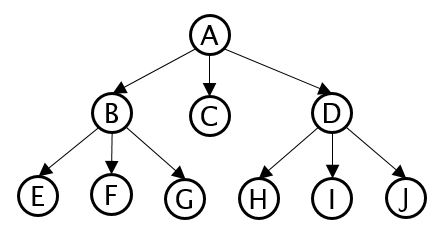
\includegraphics[width=2in]{assignment08-bsts/general-tree-no-color.png}}
\caption{\label{fig:general-tree-no-color} The given general tree.}
\end{figure}

{\bf Encoding Step 1} Redraw edges (only connect each node with its first child and also to 
the sibling to the right). To see clearly which edges will be left-going, and 
which are right-going, can color them differently. See
Figure~\ref{fig:colored-binary-tree1-reordered}. 


\begin{figure}[!htb]
\center{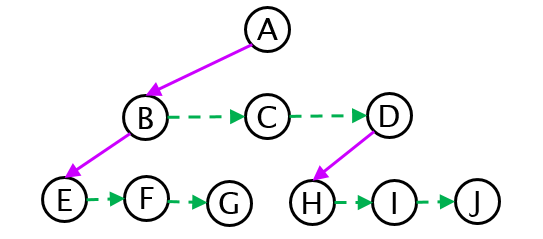
\includegraphics[width=2in]{assignment08-bsts/colored-binary-tree1-reordered.png}}
\caption{\label{fig:colored-binary-tree1-reordered} Reordering the levels.}
\end{figure}

{\bf Encoding Step 2} Adjust the levels in the new binary tree so that it takes 
a more conventional look (left children to the left, right children to the right).
See Figure~\ref{fig:colored-binary-tree1}.

\begin{figure}[!htb]
\center{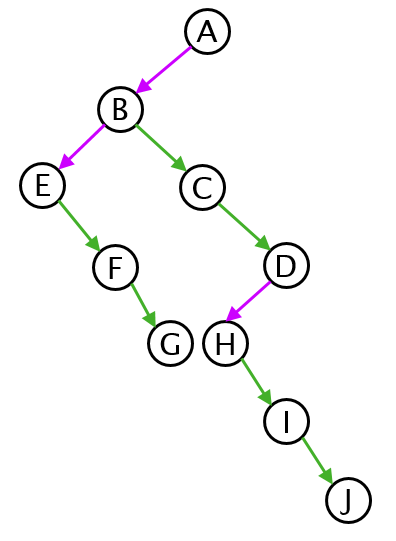
\includegraphics[width=1.5in]{assignment08-bsts/colored-binary-tree1.png}}
\caption{\label{fig:colored-binary-tree1} Binary tree with edges colored.}
\end{figure}




\vspace{10pt}
{\bf Question 1: Decode to a General Tree}

\vspace{5pt}
{\bf (A)} List all the nodes in Figure~\ref{fig:binary-tree-problem} 
using the in-order tree traversal.

\vspace{5pt}
{\bf (B)} Binary tree $B$ shown in Figure~\ref{fig:binary-tree-problem} has 
been obtained by encoding some general tree $T$ (The 
original tree $T$ was rooted 
and ordered, but it is not necessarily binary.)\\
Restore the general tree $T$ by decoding the given binary tree.

\begin{figure}[!htb]
\center{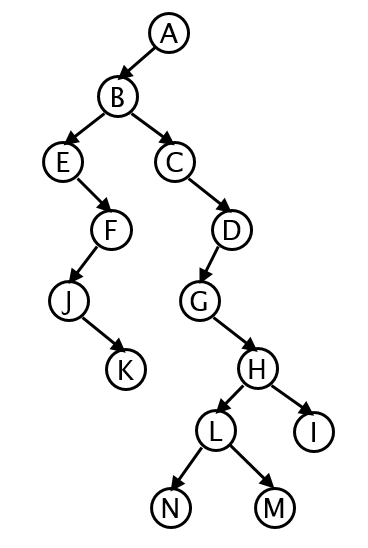
\includegraphics[width=1.5in]{assignment08-bsts/binary-tree-problem.png}}
\caption{\label{fig:binary-tree-problem} Binary tree to Convert to a General Tree}
\end{figure}









%\vspace{10pt}
%{\bf Question 2 (Run commands on a BST).}\\



\newpage


{\bf Question 1:}\\
{\bf (A)}\\
$$E,J,K,F,B,C,G,N,L,M,H,I,D,A.$$


\vspace{5pt}
{\bf (B)}\\
{\em Note.} In your answer there is no need to draw the intermediate decoding steps; 
they are just for your information. 

\vspace{5pt}
{\bf Decoding Step 1.} Can color left and right edges as 
in Figure~\ref{fig:binary-tree-problem-colored}. 

\begin{figure}[!htb]
\center{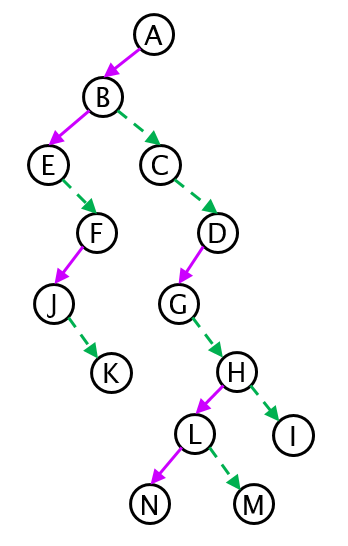
\includegraphics[width=1.5in]{assignment08-bsts/binary-tree-problem-colored.png}}
\caption{\label{fig:binary-tree-problem-colored} Colored binary tree}
\end{figure}

\vspace{5pt}
{\bf Decoding Step 2.} Now look at the previous
Figure~\ref{fig:binary-tree-problem-colored}, but 
bend your head to the right (so that the green arrows seem horizontal).

We can rearrange levels so that the right-going edges stay on the 
same level (but left-going edges go one level down). See Figure~\ref{fig:binary-tree-problem-colored-by-level}.



\begin{figure}[!htb]
\center{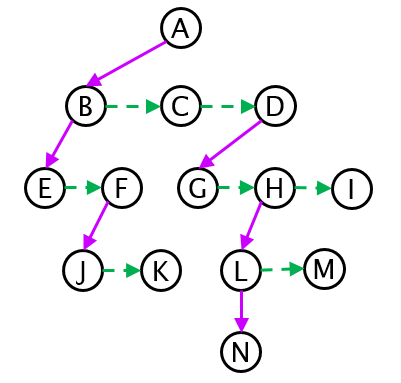
\includegraphics[width=2in]{assignment08-bsts/binary-tree-problem-colored-by-level.png}}
\caption{\label{fig:binary-tree-problem-colored-by-level} Reordered by Level}
\end{figure}


\vspace{5pt}
{\bf Decoding Step 3 (Final Answer).} Once the layers are restored, 
we can forget about the binary tree edges (the violet and green ones), 
but instead connect the parent with all the children (i.e.\ 
not just the first child, but also all its siblings to the right). 
Now the original tree is restored. See Figure~\ref{fig:binary-tree-problem-restored}.


\begin{figure}[!htb]
\center{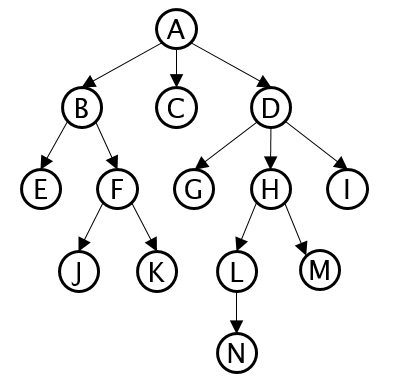
\includegraphics[width=2in]{assignment08-bsts/binary-tree-problem-restored.png}}
\caption{\label{fig:binary-tree-problem-restored} Final Answer}
\end{figure}








\end{document}



